\documentclass{standalone}
\usepackage{tikz}
\usetikzlibrary{patterns, positioning}


\begin{document}
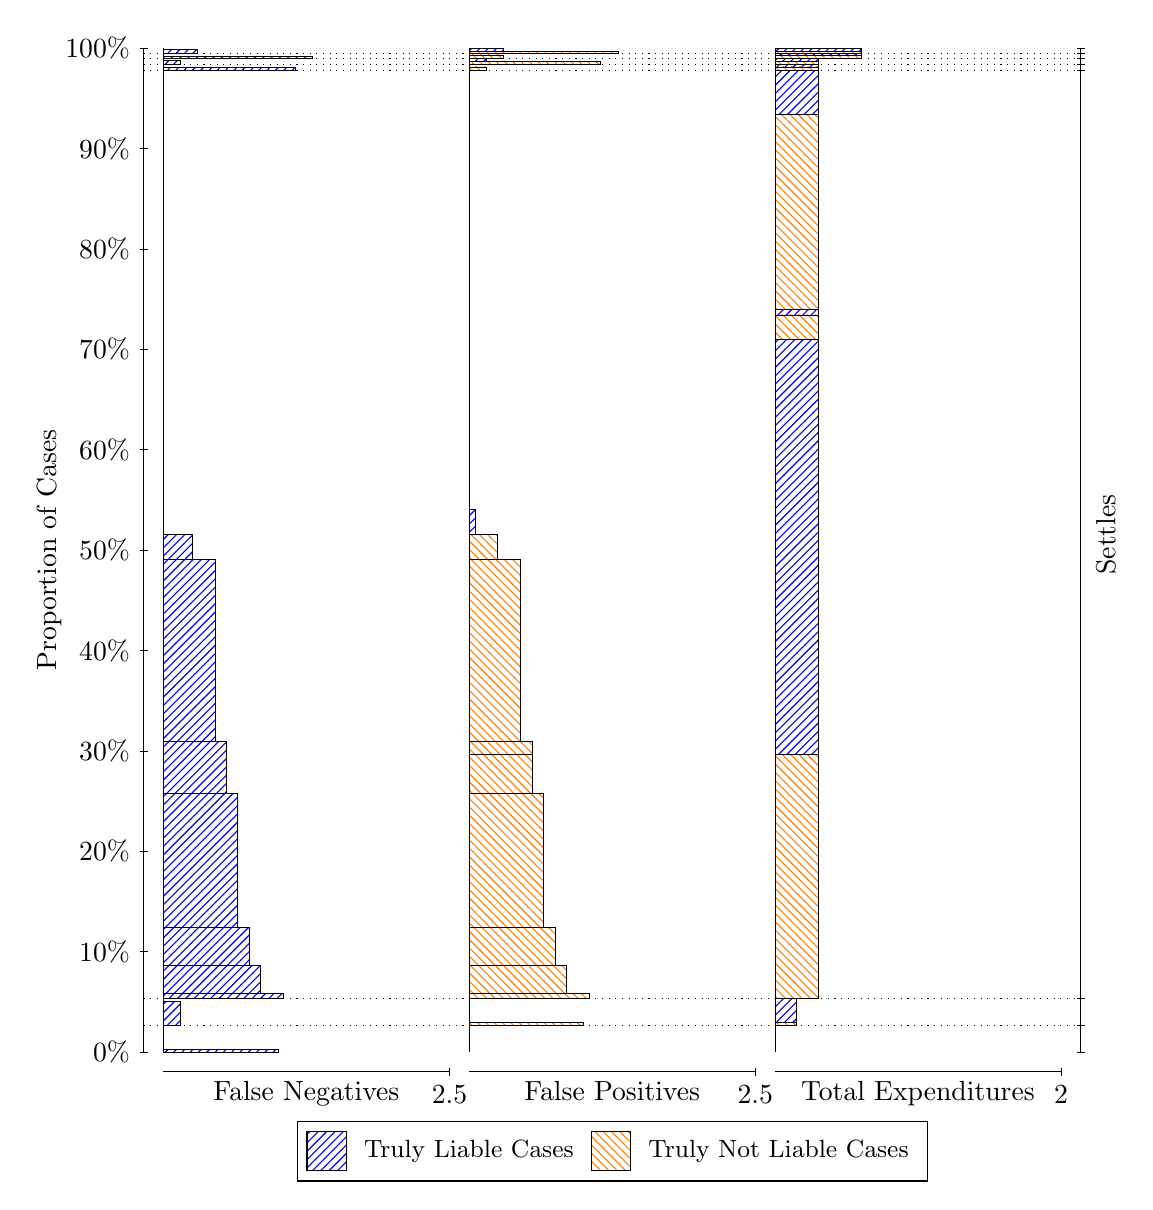
\begin{tikzpicture}
\draw[black, very thin] (1.5,1.75) -- (1.5,14.5);
\node[rotate=90, text=black, anchor=center] at (0.3, 8.125) {Proportion of Cases};
\draw[black, very thin] (1.45,1.75) -- (1.55,1.75);
\node[text=black, anchor=east] at (1.45, 1.75) {0\%};
\draw[black, very thin] (1.45,3.025) -- (1.55,3.025);
\node[text=black, anchor=east] at (1.45, 3.025) {10\%};
\draw[black, very thin] (1.45,4.3) -- (1.55,4.3);
\node[text=black, anchor=east] at (1.45, 4.3) {20\%};
\draw[black, very thin] (1.45,5.575) -- (1.55,5.575);
\node[text=black, anchor=east] at (1.45, 5.575) {30\%};
\draw[black, very thin] (1.45,6.85) -- (1.55,6.85);
\node[text=black, anchor=east] at (1.45, 6.85) {40\%};
\draw[black, very thin] (1.45,8.125) -- (1.55,8.125);
\node[text=black, anchor=east] at (1.45, 8.125) {50\%};
\draw[black, very thin] (1.45,9.4) -- (1.55,9.4);
\node[text=black, anchor=east] at (1.45, 9.4) {60\%};
\draw[black, very thin] (1.45,10.675) -- (1.55,10.675);
\node[text=black, anchor=east] at (1.45, 10.675) {70\%};
\draw[black, very thin] (1.45,11.95) -- (1.55,11.95);
\node[text=black, anchor=east] at (1.45, 11.95) {80\%};
\draw[black, very thin] (1.45,13.225) -- (1.55,13.225);
\node[text=black, anchor=east] at (1.45, 13.225) {90\%};
\draw[black, very thin] (1.45,14.5) -- (1.55,14.5);
\node[text=black, anchor=east] at (1.45, 14.5) {100\%};

\draw[black, very thin] (13.4,1.75) -- (13.4,14.5);
\draw[black, very thin] (13.35,1.75) -- (13.45,1.75);
\node[anchor=west] at (13.35, 1.75) {};
\draw[black, very thin] (13.35,2.0889) -- (13.45,2.0889);
\node[anchor=west] at (13.35, 2.0889) {};
\draw[black, very thin] (13.35,2.4278) -- (13.45,2.4278);
\node[anchor=west] at (13.35, 2.4278) {};
\draw[black, very thin] (13.35,14.217) -- (13.45,14.217);
\node[anchor=west] at (13.35, 14.217) {};
\draw[black, very thin] (13.35,14.294) -- (13.45,14.294);
\node[anchor=west] at (13.35, 14.294) {};
\draw[black, very thin] (13.35,14.371) -- (13.45,14.371);
\node[anchor=west] at (13.35, 14.371) {};
\draw[black, very thin] (13.35,14.436) -- (13.45,14.436);
\node[anchor=west] at (13.35, 14.436) {};
\draw[black, very thin] (13.35,14.5) -- (13.45,14.5);
\node[anchor=west] at (13.35, 14.5) {};

\draw[black, very thin, pattern color=blue, pattern=north east lines] (1.75,1.75) rectangle (3.2033,1.7857);
\draw[black, very thin, pattern color=orange, pattern=north west lines] (1.75,1.7857) rectangle (1.75,2.0889);
\draw[black, very thin, pattern color=blue, pattern=north east lines] (1.75,2.0889) rectangle (1.968,2.3921);
\draw[black, very thin, pattern color=orange, pattern=north west lines] (1.75,2.3921) rectangle (1.75,2.4278);
\draw[black, very thin, pattern color=blue, pattern=north east lines] (1.75,2.4278) rectangle (3.276,2.4971);
\draw[black, very thin, pattern color=blue, pattern=north east lines] (1.75,2.4971) rectangle (2.9853,2.8482);
\draw[black, very thin, pattern color=blue, pattern=north east lines] (1.75,2.8482) rectangle (2.84,3.3327);
\draw[black, very thin, pattern color=blue, pattern=north east lines] (1.75,3.3327) rectangle (2.6947,5.0335);
\draw[black, very thin, pattern color=blue, pattern=north east lines] (1.75,5.0335) rectangle (2.5493,5.6929);
\draw[black, very thin, pattern color=blue, pattern=north east lines] (1.75,5.6929) rectangle (2.404,8.0063);
\draw[black, very thin, pattern color=blue, pattern=north east lines] (1.75,8.0063) rectangle (2.1133,8.3223);
\draw[black, very thin, pattern color=orange, pattern=north west lines] (1.75,8.3223) rectangle (1.75,14.217);
\draw[black, very thin, pattern color=blue, pattern=north east lines] (1.75,14.217) rectangle (3.4213,14.25);
\draw[black, very thin, pattern color=orange, pattern=north west lines] (1.75,14.25) rectangle (1.75,14.294);
\draw[black, very thin, pattern color=blue, pattern=north east lines] (1.75,14.294) rectangle (1.968,14.339);
\draw[black, very thin, pattern color=orange, pattern=north west lines] (1.75,14.339) rectangle (1.75,14.371);
\draw[black, very thin, pattern color=blue, pattern=north east lines] (1.75,14.371) rectangle (3.6393,14.394);
\draw[black, very thin, pattern color=orange, pattern=north west lines] (1.75,14.394) rectangle (1.75,14.436);
\draw[black, very thin, pattern color=blue, pattern=north east lines] (1.75,14.436) rectangle (2.186,14.478);
\draw[black, very thin, pattern color=orange, pattern=north west lines] (1.75,14.478) rectangle (1.75,14.5);
\draw[black, very thin, pattern color=orange, pattern=north west lines] (5.6333,1.75) rectangle (5.6333,2.0533);
\draw[black, very thin, pattern color=blue, pattern=north east lines] (5.6333,2.0533) rectangle (5.6333,2.0889);
\draw[black, very thin, pattern color=orange, pattern=north west lines] (5.6333,2.0889) rectangle (7.0867,2.1246);
\draw[black, very thin, pattern color=blue, pattern=north east lines] (5.6333,2.1246) rectangle (5.6333,2.4278);
\draw[black, very thin, pattern color=orange, pattern=north west lines] (5.6333,2.4278) rectangle (7.1593,2.4971);
\draw[black, very thin, pattern color=orange, pattern=north west lines] (5.6333,2.4971) rectangle (6.8687,2.8482);
\draw[black, very thin, pattern color=orange, pattern=north west lines] (5.6333,2.8482) rectangle (6.7233,3.3327);
\draw[black, very thin, pattern color=orange, pattern=north west lines] (5.6333,3.3327) rectangle (6.578,5.0335);
\draw[black, very thin, pattern color=orange, pattern=north west lines] (5.6333,5.0335) rectangle (6.4327,5.5265);
\draw[black, very thin, pattern color=orange, pattern=north west lines] (5.6333,5.5265) rectangle (6.4327,5.693);
\draw[black, very thin, pattern color=orange, pattern=north west lines] (5.6333,5.693) rectangle (6.2873,8.0064);
\draw[black, very thin, pattern color=orange, pattern=north west lines] (5.6333,8.0064) rectangle (5.9967,8.3225);
\draw[black, very thin, pattern color=blue, pattern=north east lines] (5.6333,8.3225) rectangle (5.706,8.6385);
\draw[black, very thin, pattern color=blue, pattern=north east lines] (5.6333,8.6385) rectangle (5.6333,14.217);
\draw[black, very thin, pattern color=orange, pattern=north west lines] (5.6333,14.217) rectangle (5.8513,14.261);
\draw[black, very thin, pattern color=blue, pattern=north east lines] (5.6333,14.261) rectangle (5.6333,14.294);
\draw[black, very thin, pattern color=orange, pattern=north west lines] (5.6333,14.294) rectangle (7.3047,14.327);
\draw[black, very thin, pattern color=blue, pattern=north east lines] (5.6333,14.327) rectangle (5.8513,14.371);
\draw[black, very thin, pattern color=orange, pattern=north west lines] (5.6333,14.371) rectangle (6.0693,14.414);
\draw[black, very thin, pattern color=blue, pattern=north east lines] (5.6333,14.414) rectangle (5.6333,14.436);
\draw[black, very thin, pattern color=orange, pattern=north west lines] (5.6333,14.436) rectangle (7.5227,14.458);
\draw[black, very thin, pattern color=blue, pattern=north east lines] (5.6333,14.458) rectangle (6.0693,14.5);
\draw[black, very thin, pattern color=orange, pattern=north west lines] (9.5167,1.75) rectangle (9.5167,2.0533);
\draw[black, very thin, pattern color=blue, pattern=north east lines] (9.5167,2.0533) rectangle (9.5167,2.0889);
\draw[black, very thin, pattern color=orange, pattern=north west lines] (9.5167,2.0889) rectangle (9.7892,2.1246);
\draw[black, very thin, pattern color=blue, pattern=north east lines] (9.5167,2.1246) rectangle (9.7892,2.4278);
\draw[black, very thin, pattern color=orange, pattern=north west lines] (9.5167,2.4278) rectangle (10.062,5.5265);
\draw[black, very thin, pattern color=blue, pattern=north east lines] (9.5167,5.5265) rectangle (10.062,10.796);
\draw[black, very thin, pattern color=orange, pattern=north west lines] (9.5167,10.796) rectangle (10.062,11.112);
\draw[black, very thin, pattern color=blue, pattern=north east lines] (9.5167,11.112) rectangle (10.062,11.181);
\draw[black, very thin, pattern color=orange, pattern=north west lines] (9.5167,11.181) rectangle (10.062,13.661);
\draw[black, very thin, pattern color=blue, pattern=north east lines] (9.5167,13.661) rectangle (10.062,14.217);
\draw[black, very thin, pattern color=orange, pattern=north west lines] (9.5167,14.217) rectangle (10.062,14.261);
\draw[black, very thin, pattern color=blue, pattern=north east lines] (9.5167,14.261) rectangle (10.062,14.294);
\draw[black, very thin, pattern color=orange, pattern=north west lines] (9.5167,14.294) rectangle (10.062,14.327);
\draw[black, very thin, pattern color=blue, pattern=north east lines] (9.5167,14.327) rectangle (10.062,14.371);
\draw[black, very thin, pattern color=orange, pattern=north west lines] (9.5167,14.371) rectangle (10.607,14.414);
\draw[black, very thin, pattern color=blue, pattern=north east lines] (9.5167,14.414) rectangle (10.607,14.436);
\draw[black, very thin, pattern color=orange, pattern=north west lines] (9.5167,14.436) rectangle (10.607,14.458);
\draw[black, very thin, pattern color=blue, pattern=north east lines] (9.5167,14.458) rectangle (10.607,14.5);
\draw[black, dotted] (1.5,2.0889) -- (13.4,2.0889);
\draw[black, dotted] (1.5,2.4278) -- (13.4,2.4278);
\draw[black, dotted] (1.5,14.217) -- (13.4,14.217);
\draw[black, dotted] (1.5,14.294) -- (13.4,14.294);
\draw[black, dotted] (1.5,14.371) -- (13.4,14.371);
\draw[black, dotted] (1.5,14.436) -- (13.4,14.436);
\draw[black, very thin] (1.75,1.5) -- (5.3833,1.5);
\node[text=black, anchor=north] at (3.5667, 1.5) {False Negatives};
\draw[black, very thin] (5.3833,1.45) -- (5.3833,1.55);
\node[text=black, anchor=north] at (5.3833, 1.45) {2.5};

\draw[black, very thin] (5.6333,1.5) -- (9.2667,1.5);
\node[text=black, anchor=north] at (7.45, 1.5) {False Positives};
\draw[black, very thin] (9.2667,1.45) -- (9.2667,1.55);
\node[text=black, anchor=north] at (9.2667, 1.45) {2.5};

\draw[black, very thin] (9.5167,1.5) -- (13.15,1.5);
\node[text=black, anchor=north] at (11.333, 1.5) {Total Expenditures};
\draw[black, very thin] (13.15,1.45) -- (13.15,1.55);
\node[text=black, anchor=north] at (13.15, 1.45) {2};



\node[text=black, centered, rotate=90] at (13.72, 8.3224) {Settles};





\draw (7.449999999999999,1.5) node[draw=none] (baseCoordinate) {};
\begin{scope}[align=center]
        \matrix[scale=0.5, draw=black, below=0.5cm of baseCoordinate, nodes={draw}, column sep=0.1cm]{
            \node[rectangle, draw, minimum width=0.5cm, minimum height=0.5cm, pattern color=blue, pattern=north east lines] {}; &
            \node[draw=none, font=\small, text=black] (B) {Truly Liable Cases}; &
            \node[rectangle, draw, minimum width=0.5cm, minimum height=0.5cm, pattern color=orange, pattern=north west lines] {}; &
            \node[draw=none, font=\small, text=black] (B) {Truly Not Liable Cases}; \\
            };
\end{scope}

\end{tikzpicture}
\end{document}